\documentclass[blue,uncompressed]{beamer}
\usepackage{tikz}
\usepackage{graphicx}
\usepackage{listings}
\usepackage[english]{babel}
\usepackage[utf8]{inputenc}
\usepackage[scale=0.82]{FiraMono}
\usepackage[T1]{fontenc}
\usepackage{multirow}
\usepackage[gen]{eurosym}   % For \euro{} symbol
\pdfinfo
{
  /Title       (Introduction to High Performance Computing with SYCL)
  /Creator     (Adriano dos Santos Moreira)
  /Author      (Adriano dos Santos Moreira)
  /Subject     (Trabajo de Fin de Grado)
}
%%%%%%%%%%%%%%%%%%%%%%%%%%%%%%%%%%%%%%%%%%%%%%%%%%%%%%%%%%%%%%%%%%%%%%%%%%%%%%%%%%%%%%%%%%
% Definiendo colores para los listados de código fuente - Univ. Deusto
% \definecolor{violet}{rgb}{0.5,0,0.5}
% \definecolor{navy}{rgb}{0,0,0.5}
% \definecolor{hellgelb}{rgb}{1,1,0.8}
\definecolor{colKeys}{rgb}{0,0,53}           %%% Todo : check color for keys
\definecolor{colIdentifier}{rgb}{0,0,0}
\definecolor{colString}{rgb}{0,0.5,0}
\definecolor{lightlightgray}{rgb}{204,204,204}
\definecolor{darkgray}{rgb}{.4,.4,.4}
\definecolor{main-color}{rgb}{0,0,0}
\definecolor{back-color}{rgb}{0.1686, 0.1686, 0.1686}
\definecolor{string-color}{HTML}{953800}
\definecolor{key-color}{HTML}{8250DF}
\definecolor{comment-color}{HTML}{008000}
\definecolor{sycl-color}{HTML}{CF222E}
\definecolor{highlight-color}{HTML}{953800}
%%%%%%%%%%%%%%%%%%%%%%%%%%%%%%%%%%%%%%%%%%%%%%%%%%%%%%%%%%%%%%%%%%%%%%%%%%%%%%%%%%%%%%%%
\lstloadlanguages{Java}
\lstloadlanguages{XML} 
\lstset{
	float=hbp,
		language = Java,
			morekeywords={hicuda,global,alloc,shape,kernel,thread,loop_partition,tblock,over_tblock,over_thread,kernel_end,copyout,free,data,region,task,input,inout,output,pragma,omp,parallel,reduction,private,shared,target,device,copy_in,copy_out,acc,kernels,loop,copyin,copy,pcopy,pcopyin,collapse,gang,worker,independent,firstprivate,endfor,in},
				%\emph      ={omp,parallel,reduction,private,shared},
				xleftmargin=5.0ex,    % Margen izq. para que los números de línea se vean
				emphstyle=\textbf,
        basicstyle=\ttfamily\scriptsize,
        identifierstyle=\color{colIdentifier},
        keywordstyle=\color{colKeys},
        stringstyle=\color{colString},
        commentstyle=\color[rgb]{0.133,0.545,0.133},
        columns=flexible,
        tabsize=4,
        frame=single,
        extendedchars=true,
        showspaces=false,
        showstringspaces=false,
        numbers=left,
        numberstyle=\tiny,
        breaklines=true,
        backgroundcolor=\color{lightlightgray},
        breakautoindent=true,
        captionpos=b
        morecomment=[l][\color{colKeys}]{\#}
}

\lstdefinelanguage{C++}{
  keywords={new, true, false, catch, try, return, null, switch, const, if, in, while, do, else, case, break},
  ndkeywords={class, throw, this},
  sensitive=false,
  comment=[l]{//},
  morecomment=[s]{/*}{*/},
  morestring=[b]',
  morestring=[b]"
}

\lstdefinestyle{cppstyle}{
    language=C++,
    basicstyle = {\ttfamily\color{main-color}\scriptsize},
    backgroundcolor = {\color{back-color}},
    stringstyle = {\color{string-color}},
    keywordstyle = {\color{key-color}},
    keywordstyle = [2]{\color{gray}},
    keywordstyle = [3]{\color{sycl-color}},
    keywordstyle = [4]{\color{highlight-color}},
    keywordstyle = [5]{\color{black}},
    commentstyle = {\color{comment-color}},
    otherkeywords = {++,--,<<,>>,<<<,>>>,+,-,\{,\},\[,\],*,\&,sycl,std},
    morekeywords = [2]{++,--,<<,>>},
    morekeywords = [3]{sycl},
    morekeywords = [4]{std,+,-,{,},[,],*,\&},
    morekeywords = [5]{<<<,>>>},
    columns=flexible,
    tabsize=2,
    frame=single,
    extendedchars=true,
    showspaces=false,
    showstringspaces=false,
    numbers=left,
    numberstyle=\tiny,
    breaklines=true,
    backgroundcolor=\color{white},
    breakautoindent=true,
    captionpos=b
}

\lstset{literate=%
   *{0}{{{\color{darkgray}0}}}1
    {1}{{{\color{darkgray}1}}}1
    {2}{{{\color{darkgray}2}}}1
    {3}{{{\color{darkgray}3}}}1
    {4}{{{\color{darkgray}4}}}1
    {5}{{{\color{darkgray}5}}}1
    {6}{{{\color{darkgray}6}}}1
    {7}{{{\color{darkgray}7}}}1
    {8}{{{\color{darkgray}8}}}1
    {9}{{{\color{darkgray}9}}}1
} 
%%%%%%%%%%%%%%%%%%%%%%%%%%%%%%%%%%%%%%%%%%%%%%%%%%%%%%%%%%%%%%%%%%%%%%%%%%%%%%%%%%%%%%%%%%%%
\mode<handout>
{ 
	\usepackage{pgfpages}
	\pgfpagesuselayout{2 on 1}[a4paper,border shrink=5mm]
	\setbeamercolor{background canvas}{bg=black!0}
	\setbeameroption{show notes}
}

\mode<presentation>
{
	\usetheme{Madrid}
	\usecolortheme{ull}
	\setbeamercovered{transparent}
	%\logo{  % Logo ULL en esquina inferior derecha
	%    \includegraphics[width=.25\textwidth]{FIGURES/logoull-oficial.png}
	%}
}

\makeatletter
\setbeamertemplate{footline}
{
  \leavevmode%
  \hbox{%
  \begin{beamercolorbox}[wd=.333333\paperwidth,ht=2.25ex,dp=1ex,center]{author in head/foot}%
    \usebeamerfont{author in head/foot}\insertshortauthor%~~\beamer@ifempty{\insertshortinstitute}{}{(\insertshortinstitute)}
  \end{beamercolorbox}%
  \begin{beamercolorbox}[wd=.333333\paperwidth,ht=2.25ex,dp=1ex,center]{title in head/foot}%
    \usebeamerfont{title in head/foot}\insertshorttitle
  \end{beamercolorbox}%
  \begin{beamercolorbox}[wd=.333333\paperwidth,ht=2.25ex,dp=1ex,right]{date in head/foot}%
    \usebeamerfont{date in head/foot}\insertshortdate{}\hspace*{2em}
    \insertframenumber{} / \inserttotalframenumber\hspace*{2ex} 
  \end{beamercolorbox}}%
  \vskip0pt%
}
\makeatother

%%%%%%%%%%%%%%%%%%%%%%%%%%%%%%%%%%%%%%%%%%%%%%%%%%%%%%%%%%%%%%%%%%%%%%%%%%%%%%%%%%%%%%%%%%
\AtBeginSection[]
{
	\begin{frame}<beamer>
		\frametitle{Outline}
		\tableofcontents[currentsection,currentsubsection]
	\end{frame}
} 
%%%%%%%%%%%%%%%%%%%%%%%%%%%%%%%%%%%%%%%%%%%%%%%%%%%%%%%%%%%%%%%%%%%%%%%%%%%%%%%%%%%%%%%%%%
\title{\textbf{HPC with SYCL}}
\subtitle{Introduction to High Performance Computing with SYCL}
\author[Adriano dos Santos Moreira]
{
	\textbf{Adriano dos Santos Moreira} \\ \textbf{Advisor}: Francisco de Sande González \\ \textbf{Co-advisor}: Alberto Cabrera Pérez (Codeplay Software Ltd.)
}

\institute[ULL]

\date[Trabajo de Fin de Grado]{\textsc{Trabajo de Fin de Grado}     \\
                           La Laguna, 16 de Julio, 2024}
\subject{TFG}

\AtBeginSection[]
{
	\frame<handout:0>
		{
			\frametitle{Índice}
			\tableofcontents[current]
		}
}
%%%%%%%%%%%%%%%%%%%%%%%%%%%%%%%%%%%%%%%%%%%%%%%%%%%%%%%%%%%%%%%%%%%%
\newcommand{\ULLAR}{\texttt{ULL-AR{}}}
\setbeamerfont{title}{size=\Large,shape=\sffamily}
\setbeamerfont{author}{size=\small,shape=\sffamily}
\setbeamerfont{institute}{size=\scriptsize,shape=\sffamily}
\setbeamerfont{date}{size=\scriptsize,shape=\sffamily}
%%%%%%%%%%%%%%%%%%%%%%%% Title Page %%%%%%%%%%%%%%%%%%%%%%%%%%%%%%%%
\defbeamertemplate*{title page}{AGH}[1][]
{
  \vbox{}
  %\vspace*{2.3cm}
  \vfill 
\includegraphics[width=0.4\linewidth]{Images/marca-universidad-de-la-laguna-original}
    \vfill
  %\hspace*{1.8cm}
  % \begin{columns}
  %   \begin{column}{0.6\textwidth}
      \begin{beamercolorbox}[sep=8pt,#1]{title}
	\centering{\usebeamerfont{title}\inserttitle\par}
	\ifx\insertsubtitle\@empty%
	\else%
	  \vskip0.25em%
	  {\usebeamerfont{subtitle}\usebeamercolor[fg]{subtitle}\insertsubtitle\par}%
	\fi%
	
      \end{beamercolorbox}%
      \vskip1em\par

      \begin{beamercolorbox}[sep=8pt,#1]{author}
				\centering{\usebeamerfont{author}\insertauthor}
      \end{beamercolorbox}
      \vskip1em\par
      \hspace*{3cm}
      \begin{beamercolorbox}[sep=8pt,#1]{institute}
				\centering{\usebeamerfont{institute}\insertinstitute}
      \end{beamercolorbox}
      \hspace*{3cm}
      \begin{beamercolorbox}[sep=8pt,#1]{date}
				\centering{\usebeamerfont{date}\insertdate}
      \end{beamercolorbox}\vskip0.5em
    % \end{column}
    
  %   \begin{column}{0.4\textwidth}
  %     \hfill \includegraphics[width=0.8\linewidth]{Images/App/menuPrincipal.png}
  %   \end{column}
  % \end{columns}
    %\hfill \includegraphics[width=0.2\linewidth]{Images/varios/MainActivity.png}
    %{\usebeamercolor[fg]{titlegraphic}\inserttitlegraphic\par}
	%	\vfill \includegraphics[width=0.3\linewidth]{FIGURES/logos/nwo}
	%	\hfill \includegraphics[width=0.17\linewidth]{FIGURES/logos/stw}
	%	\hfill \includegraphics[width=0.2\linewidth]{FIGURES/logos/ipn.jpg}
  %\vfill
}
%%%%%%%%%%%%%%%%%%%%%%%%%%%%%%%%%%%%%%%%%%%%%%%%%%%%%%%%%%%%%%%%%%%%%%%%%%%%%%%%%%%%%%%%%%%%
% Slide numbers. 
%\expandafter\def\expandafter\insertshorttitle\expandafter{%
%  \insertshorttitle\hfill%
%  \insertframenumber\,/\,\inserttotalframenumber
%}
%%%%%%%%%%%%%%%%%%%%%%%%%%%%%%%%%%%%%%%%%%%%%%%%%%%%%%%%%%%%%%%%%%%%%%%%%%%%%%%%%%%%%%%%%
\begin{document}
	%\frame{\titlepage}
	\begin{frame}[plain]
	\titlepage
	\end{frame}

	\frame{\frametitle{Index}\tableofcontents}
  \section{Introduction}
  % -------------------------------------------------------------------------
\begin{frame}{Introduction}
\begin{center}
\block{XXX}
\begin{itemize}
  \item XXX
\end{itemize}
\endblock{}
\begin{figure}[H]
	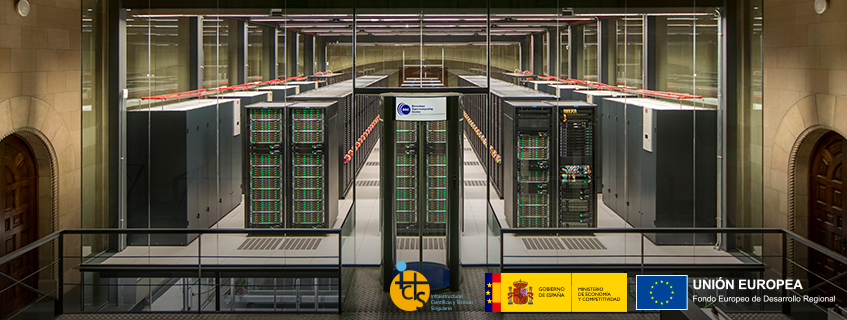
\includegraphics[width=0.65\linewidth]{Images/mare-nostrum.png}
\end{figure}
MareNostrum supercomputer in Barcelona. \textit{(Credit: \url{www.bsc.es})}
\end{center}
\end{frame}
% -------------------------------------------------------------------------
\begin{frame}{Introduction}
\begin{center}
\block{Motivation \& Objectives}
\begin{itemize}
  \item Gain knowledge in XXX 
  \item Learn about XXX
  \item Study and apply XXX
\end{itemize}
\endblock{}
\end{center}
\end{frame}
% -------------------------------------------------------------------------
\begin{frame}{Introduction}
  Nowadays, there is a wide variety of devices specialized in different types of computing tasks (CPU, FPGA, GPU, ASIC, etc.)
\begin{block}{}
With the vast amount of devices comes the also varied collection of APIs
\end{block}
\begin{center}
	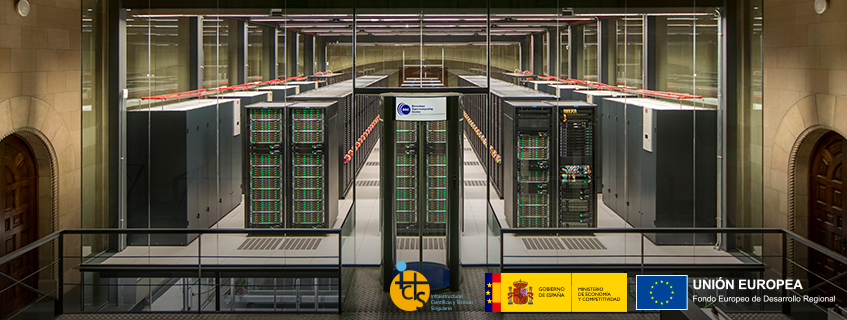
\includegraphics[width=0.65\linewidth]{Images/mare-nostrum.png}
\end{center}
\end{frame}  
% -------------------------------------------------------------------------

  \section{SYCL}
  % -------------------------------------------------------------------------
\begin{frame}{SYCL}
% \begin{center}
SYCL is a \textbf{parallel focused} abstraction layer created for C++

Characteristics:
\begin{columns}
  \begin{column}{0.48\textwidth}
    \begin{itemize}
      \item High-level
      \item Standard and modern C++
      \item Single source
      \item Portable code \\~\\
    \end{itemize}
  \end{column}
  \begin{column}{0.48\textwidth}
    \begin{center}
      
\includegraphics[width=0.7\linewidth]{Images/sycl-logo.png}
    \end{center}
  \end{column}
\end{columns}
\block{}
\begin{center}
  Targets a range of heterogeneous devices and backends
\end{center}
\endblock{}
\end{frame}
% -------------------------------------------------------------------------
\begin{frame}{SYCL}
\begin{center}
\begin{figure}[H]
  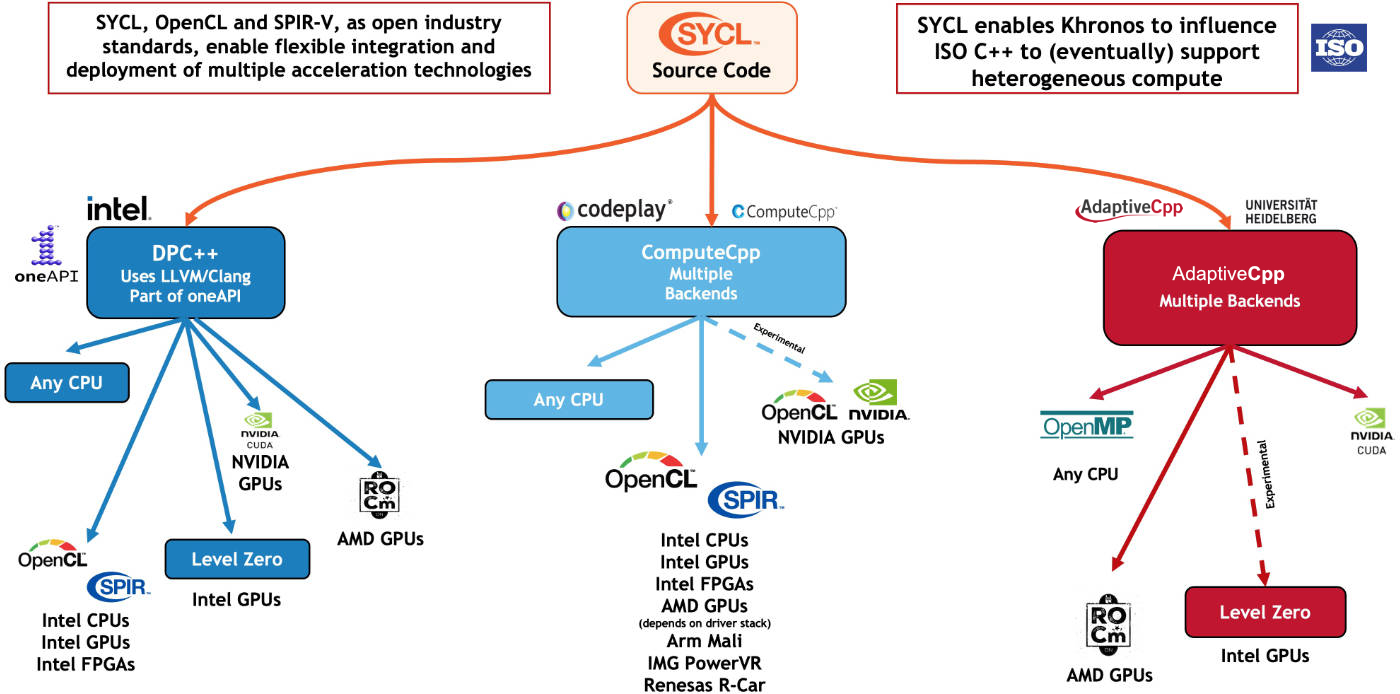
\includegraphics[width=\linewidth]{Images/sycl-map.png}
\end{figure}
SYCL backends map. \textit{(Credit: \url{www.khronos.org})}
\end{center}
\end{frame}
% -------------------------------------------------------------------------
\begin{frame}{SYCL}
  SYCL learning resources used:
\begin{columns}
  \begin{column}{0.48\textwidth}
    \begin{center}
    
\includegraphics[width=0.6\linewidth]{Images/data-parallel-cpp.png}

    Extensive book on SYCL
    \end{center}
  \end{column}
  \begin{column}{0.385\textwidth}
    \begin{center}
    
\includegraphics[width=0.7\linewidth]{Images/sycl-academy.png}
    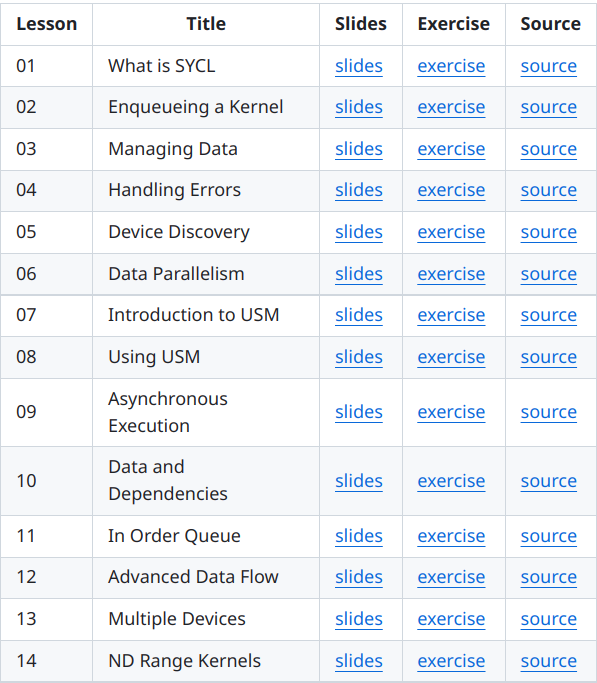
\includegraphics[width=0.9\linewidth]{Images/lessons.png}

    Practical tutorial lessons
    \end{center}
  \end{column}
\end{columns}
\end{frame}
% -------------------------------------------------------------------------
\begin{frame}{SYCL}
\begin{columns}
  \begin{column}{0.7\textwidth}
    \centering
  \lstinputlisting[language=C++,style=cppstyle]{Code/scalar_add.cc}
Scalar add. \href{{https://github.com/AdrianoMoreira08/TFG-SYCL/blob/main/sycl-examples/scalar_add.cc}}{\textit{See on Github}}
\end{column}
\begin{column}{0.3\textwidth}
  \begin{enumerate}
    \item Queue creation
    \item Buffer definition
    \item Command Group
    \begin{enumerate}
      \item Accessors
      \item Kernel
    \end{enumerate}
\end{enumerate}
\end{column}
\end{columns}
\end{frame}
% -------------------------------------------------------------------------
\begin{frame}{SYCL}
  \begin{figure}[H]
  \centering
  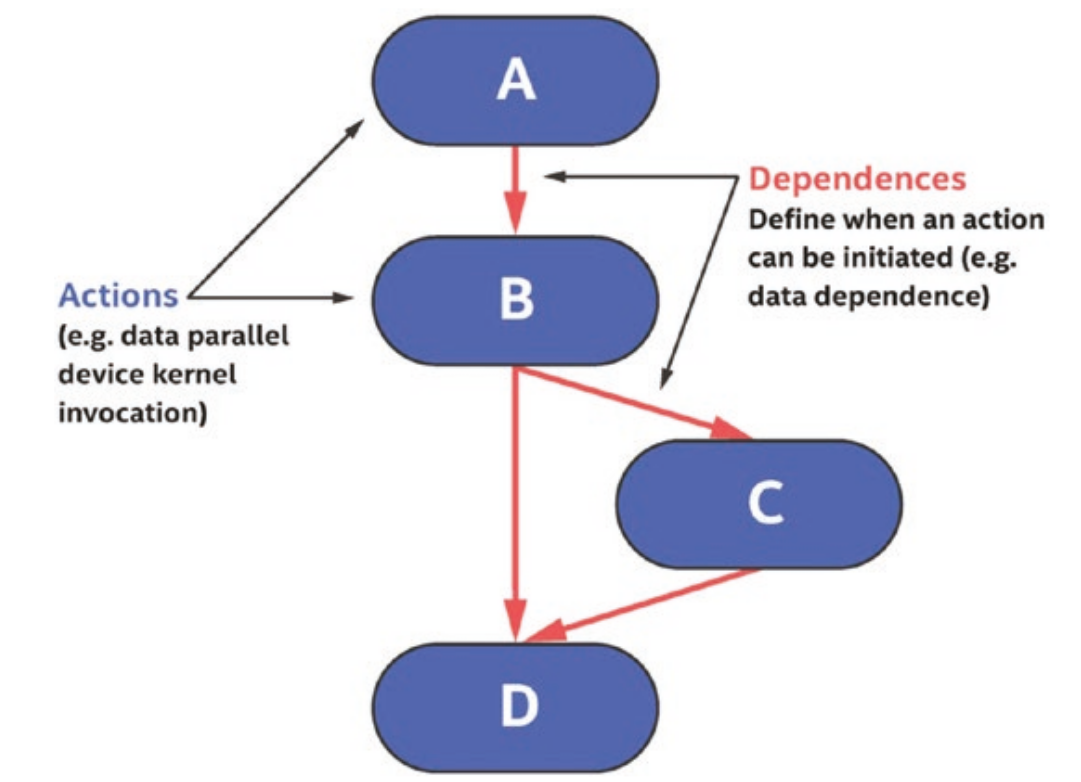
\includegraphics[width=0.74\linewidth]{Images/dependency-graph.png}

  Dependency graph example. \textit{Image From Data Parallel C++}
\end{figure}
\end{frame}
% -------------------------------------------------------------------------
\begin{frame}{SYCL}
  \begin{columns}
    \begin{column}{0.7\textwidth}
      \centering
    \lstinputlisting[language=C++,style=cppstyle]{Code/scalar_add.cc}
  Scalar add. \href{{https://github.com/AdrianoMoreira08/TFG-SYCL/blob/main/sycl-examples/scalar_add.cc}}{\textit{See on Github}}
  \end{column}
  \begin{column}{0.3\textwidth}
    \begin{enumerate}
      \item Queue creation
      \item Buffer definition
      \item Command Group
      \begin{enumerate}
        \item Accessors
        \item Kernel
      \end{enumerate}
  \end{enumerate}
  \end{column}
  \end{columns}
  \end{frame}
  % -------------------------------------------------------------------------
\begin{frame}{SYCL}
  \begin{figure}[H]
    \centering
    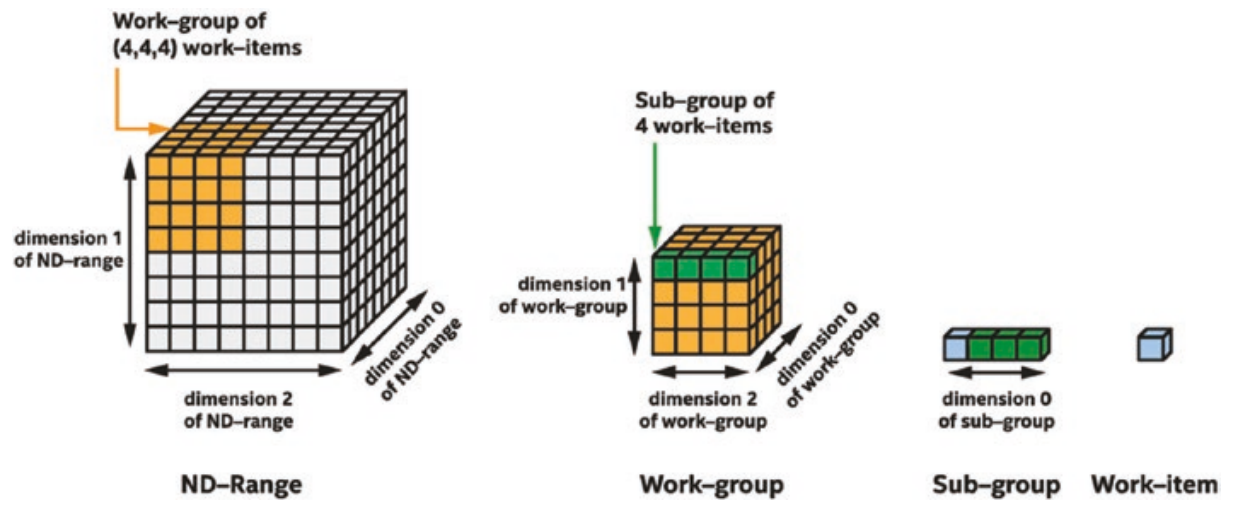
\includegraphics[width=\linewidth]{Images/nd_range.png}
    Dissection of an NDRange. \textit{From Data Parallel C++}
  \end{figure}
\end{frame}

  \section{Benchmark Comparisons}
  % -------------------------------------------------------------------------
\begin{frame}{Benchmark Comparisons}
  We will compare \textbf{serial}, \textbf{SYCL} and \textbf{CUDA} executions
\begin{block}{}
\begin{columns}[onlytextwidth]
  \column{12mm}
  
\includegraphics[width=10mm]{Images/github-logo.png}
  \column{\linewidth}
  {\large\textbf{HeCBench}}
  
  A collection of heterogeneous computing benchmarks

  \url{https://github.com/zjin-lcf/HeCBench/}
\end{columns}
\end{block}
Execution in \textit{Verode}, platform from the ULL GCAP research group (\textit{High
Performance Computing Group}). Specifications:
\begin{itemize}
  \item Two Intel\textsuperscript{\textregistered} Xeon\textsuperscript{\textregistered} CPU Gold 6230N
  \item NVIDIA Tesla V100 GPU
  \item Debian GNU/Linux 11 (bullseye)
\end{itemize}
\end{frame}
% -------------------------------------------------------------------------
\begin{frame}{Benchmark Comparisons: Mandelbrot set}
  \begin{center}
  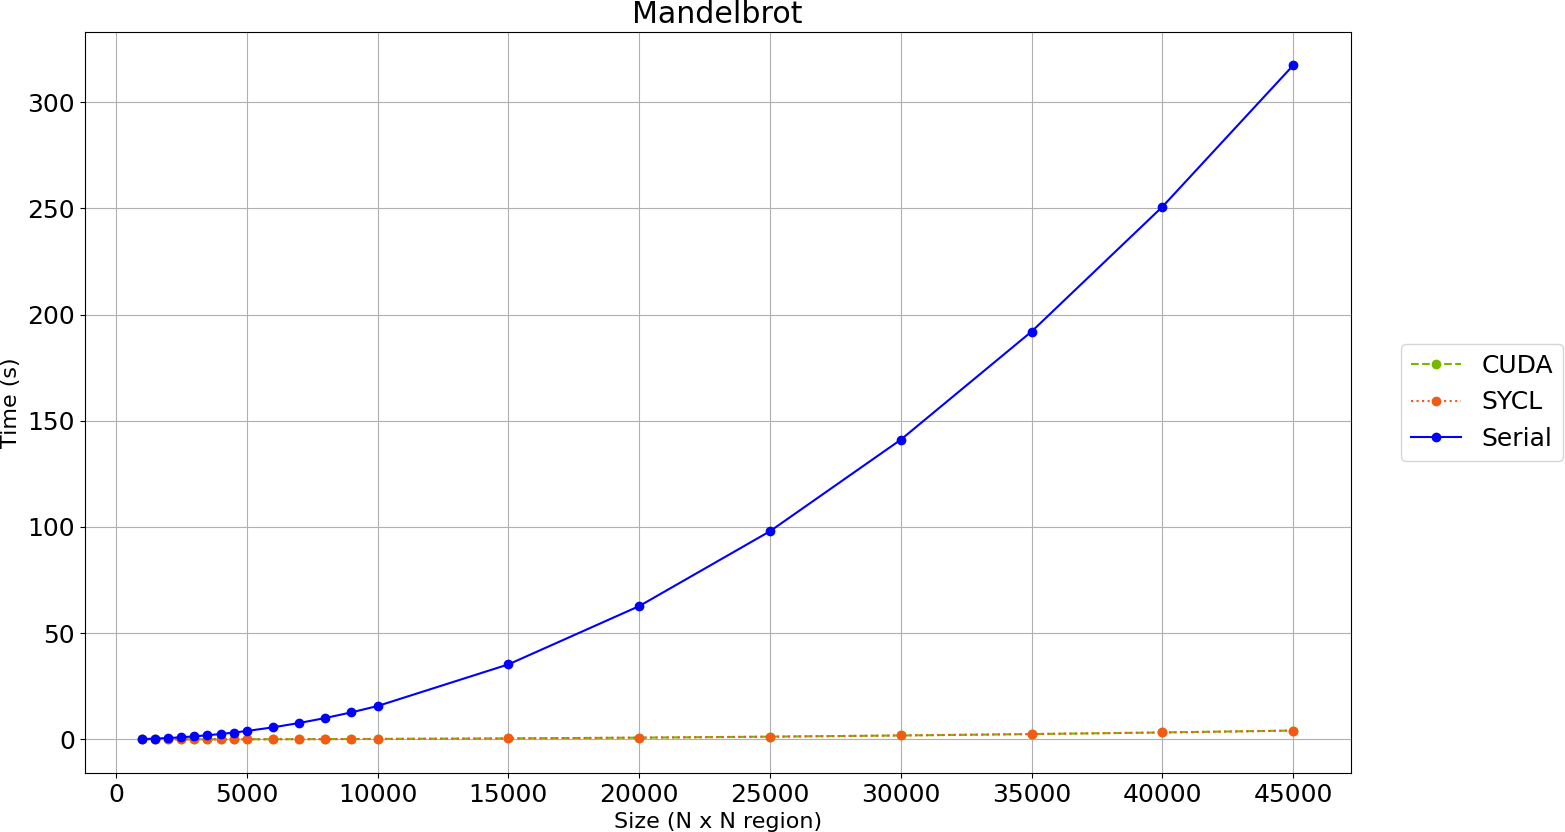
\includegraphics[width=\textwidth]{Images/mandelbrot-sycl-cuda-serial.png}
  \end{center}
\end{frame}
% -------------------------------------------------------------------------
\begin{frame}{Benchmark Comparisons: Mandelbrot set}
  \begin{center}
  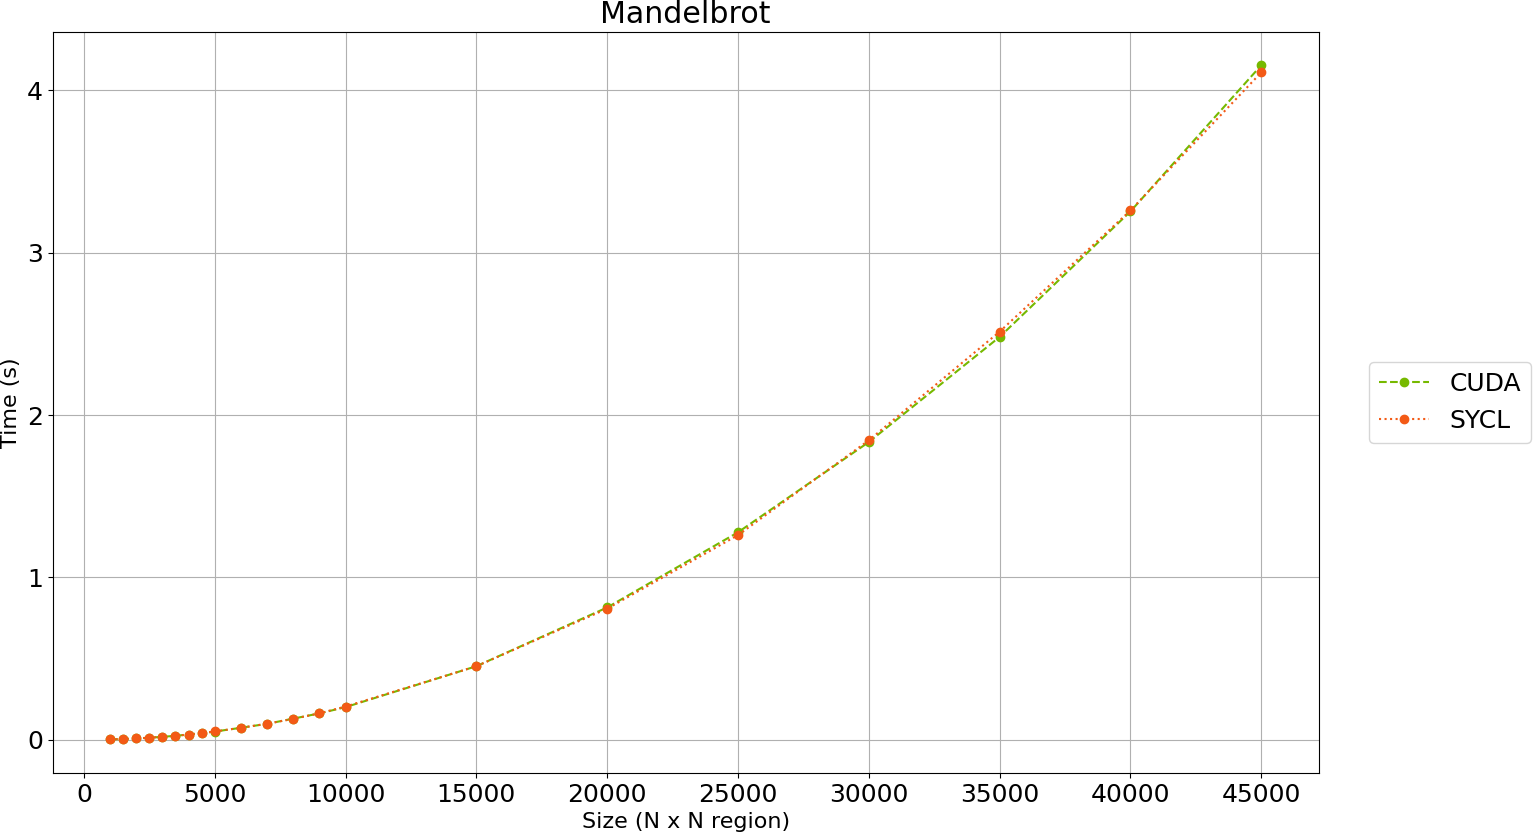
\includegraphics[width=\textwidth]{Images/mandelbrot-sycl-cuda.png}
  \end{center}
\end{frame}
% -------------------------------------------------------------------------
\begin{frame}{Benchmark Comparisons: Mandelbrot set}
  \begin{center}
  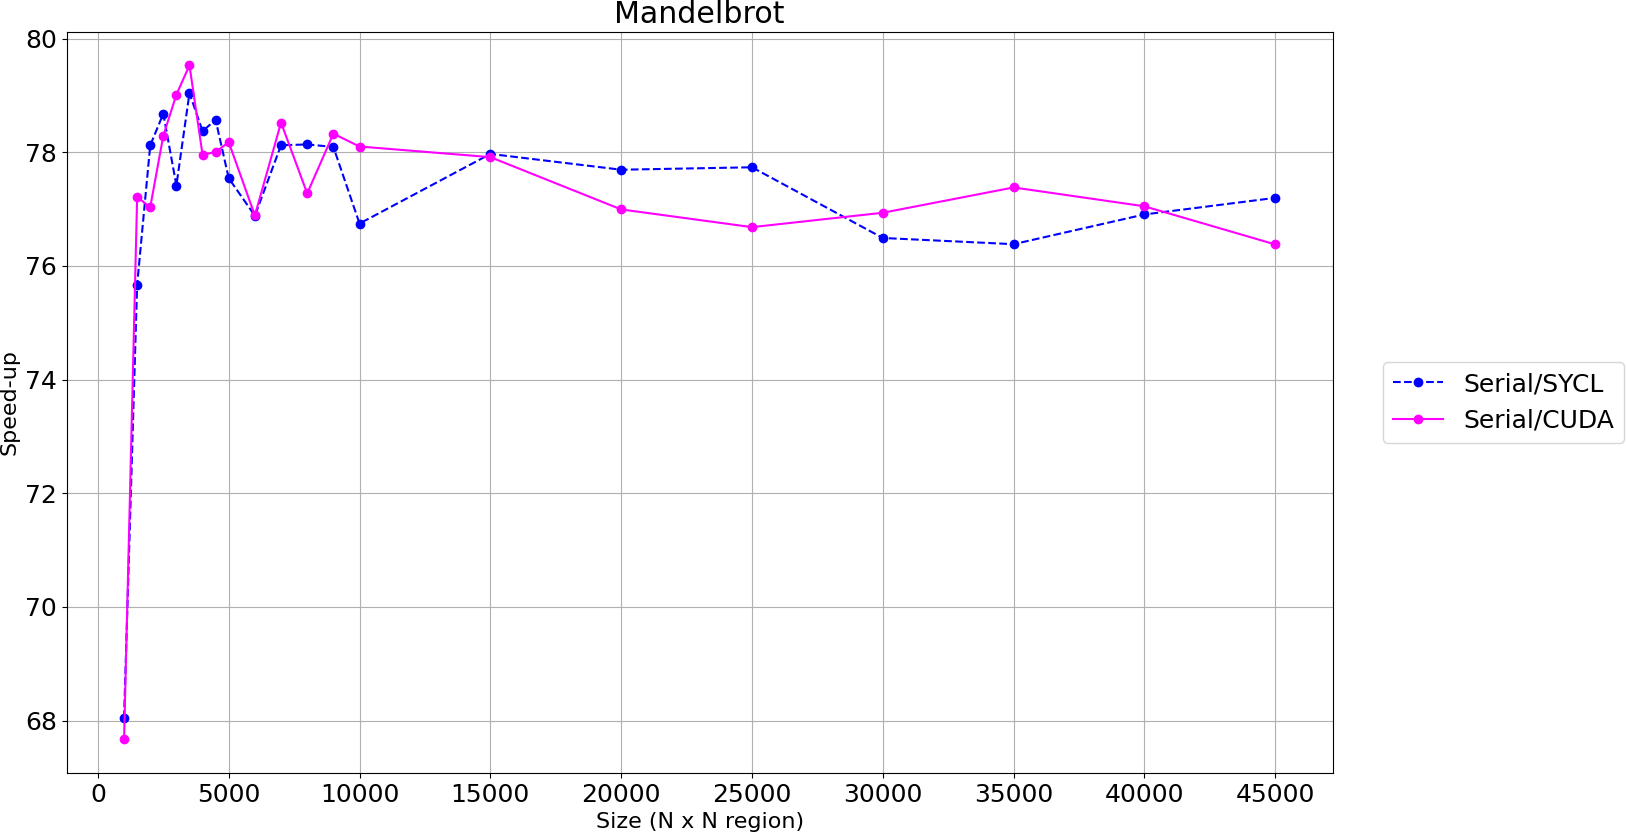
\includegraphics[width=\textwidth]{Images/mandelbrot-speed-up-sycl-cuda.png}
  \end{center}
\end{frame}
% -------------------------------------------------------------------------
\begin{frame}{Benchmark Comparisons: Floyd-Warshall algorithm}
  \begin{center}
  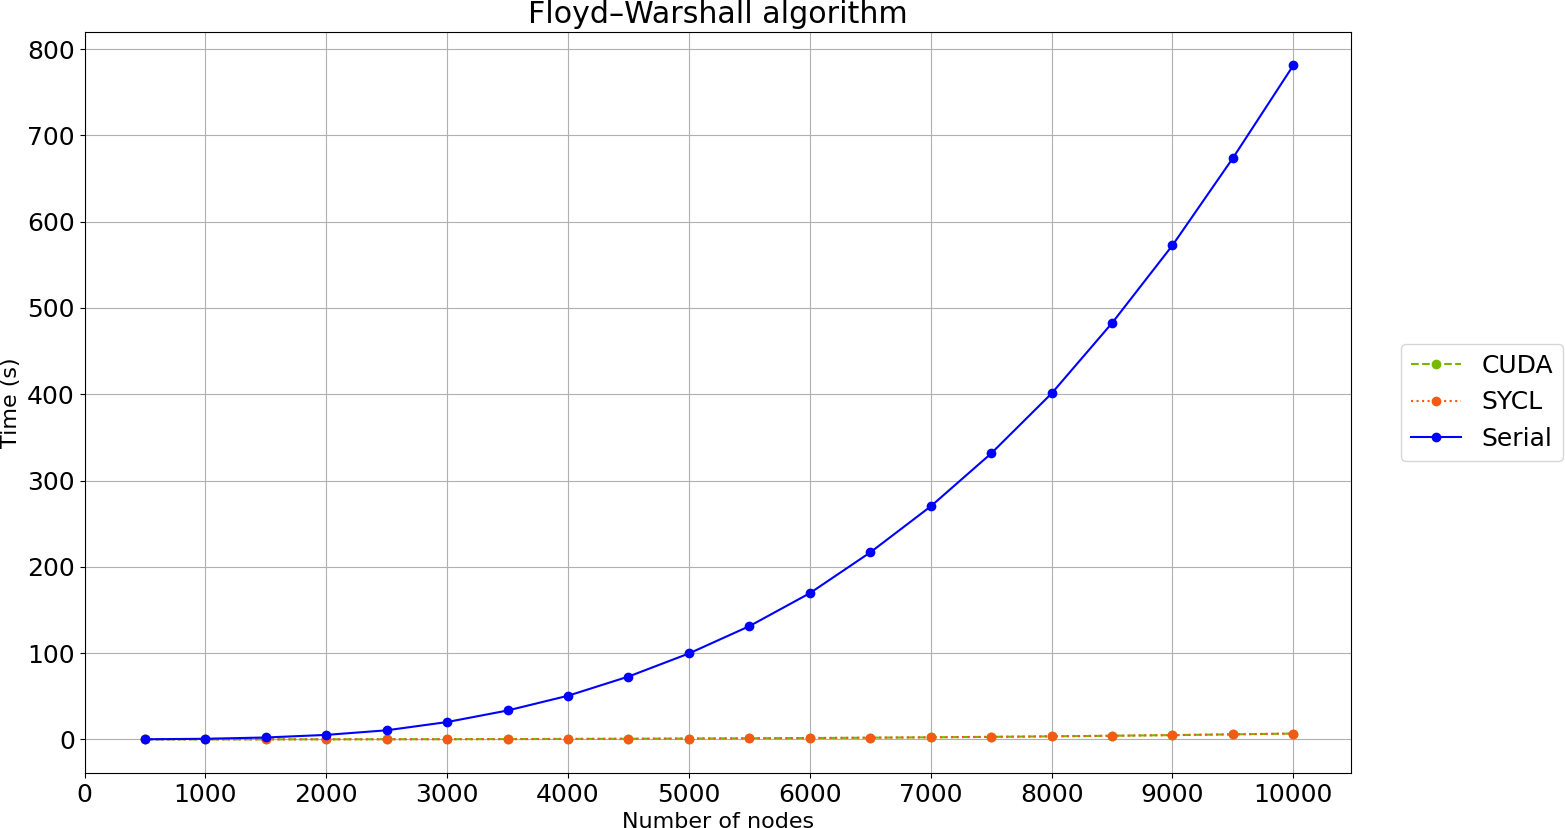
\includegraphics[width=\textwidth]{Images/floydwarshall-sycl-cuda-serial.png}
  \end{center}
\end{frame}
% -------------------------------------------------------------------------
\begin{frame}{Benchmark Comparisons: Floyd-Warshall algorithm}
  \begin{center}
  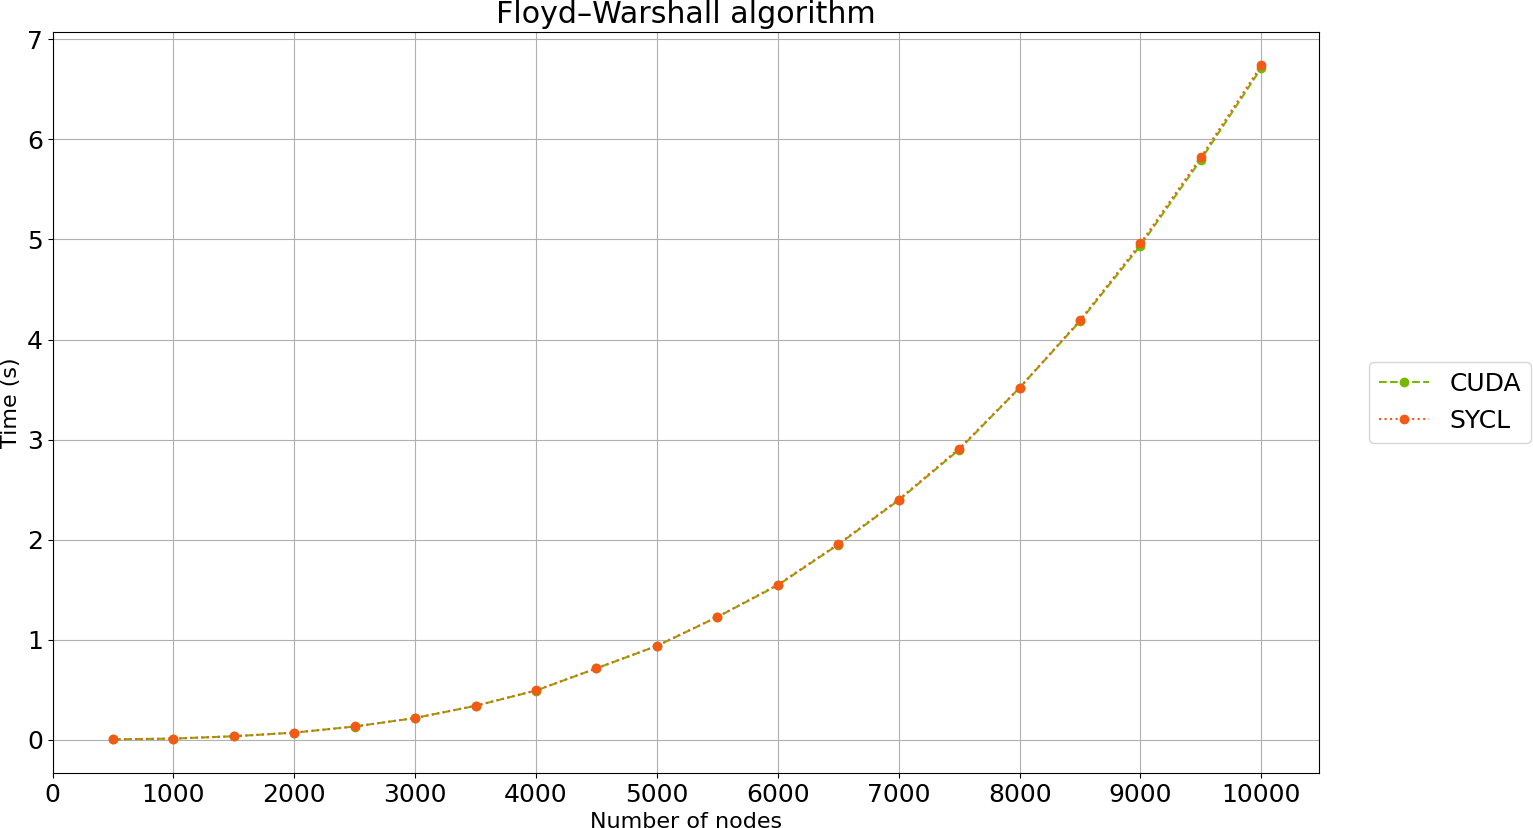
\includegraphics[width=\textwidth]{Images/floydwarshall-sycl-cuda.png}
  \end{center}
\end{frame}
% -------------------------------------------------------------------------
\begin{frame}{Benchmark Comparisons: Floyd-Warshall algorithm}
  \begin{center}
  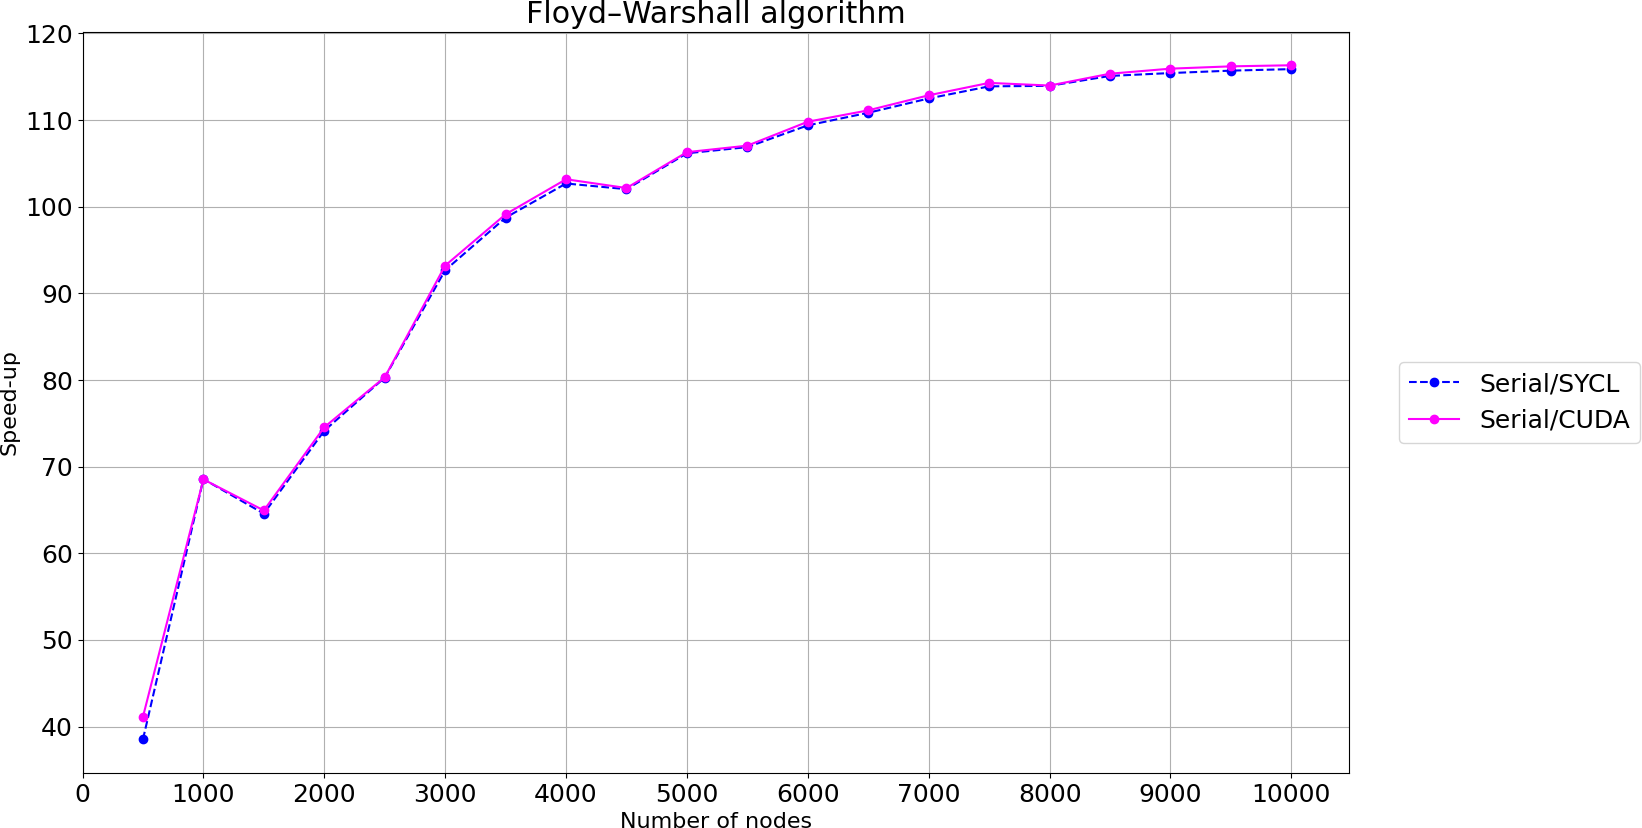
\includegraphics[width=\textwidth]{Images/floydwarshall-speed-up-sycl-cuda.png}
  \end{center}
\end{frame}
% -------------------------------------------------------------------------
\begin{frame}{Benchmark Comparisons: Molecular dynamics}
  \begin{center}
    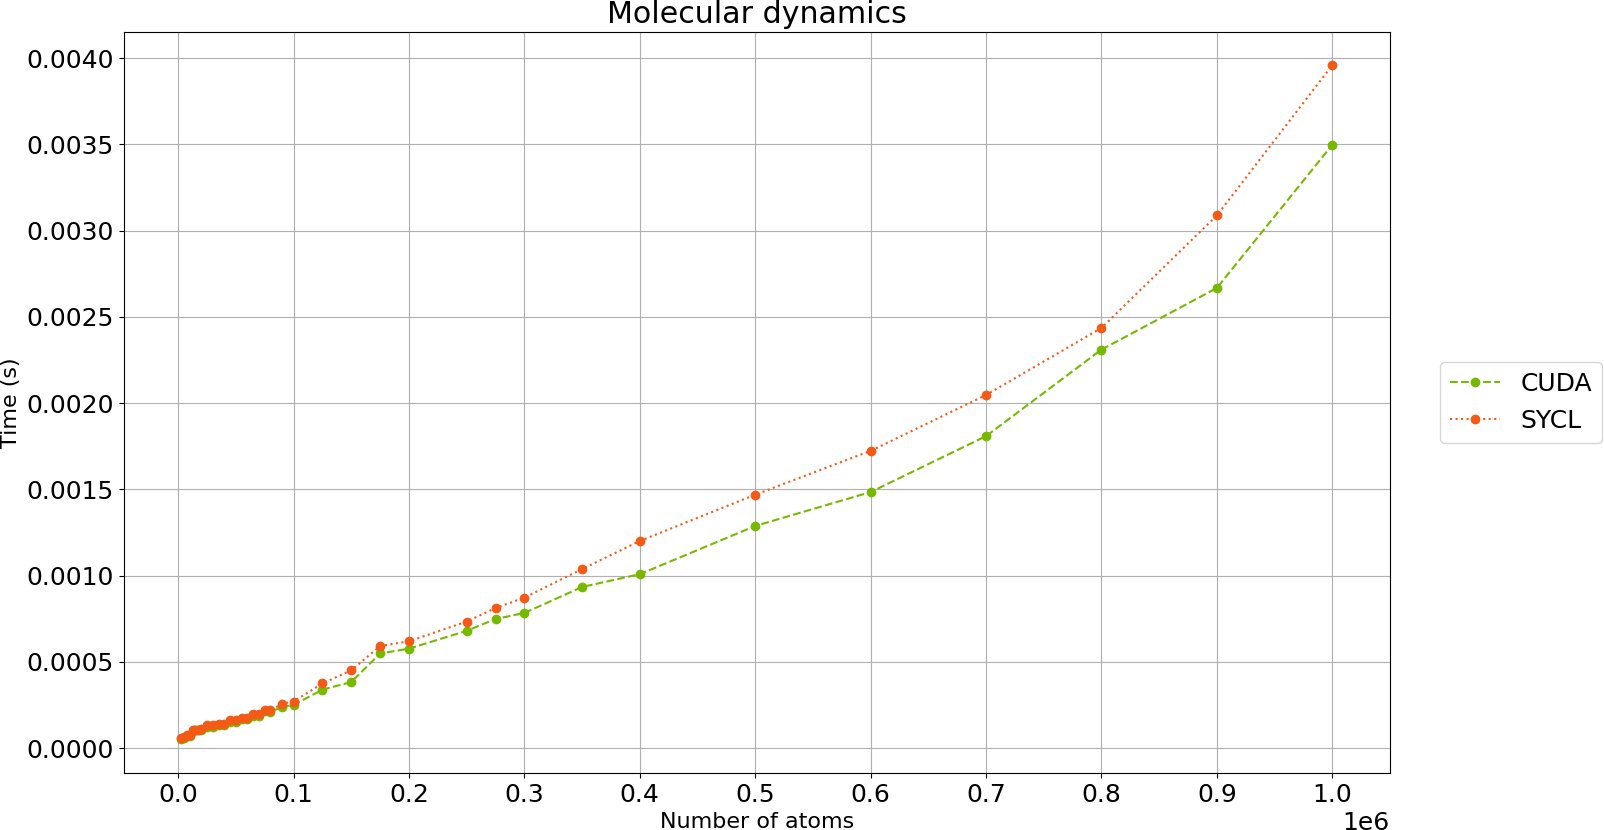
\includegraphics[width=\textwidth]{Images/md-sycl-cuda.png}
  \end{center}
\end{frame}
% -------------------------------------------------------------------------
\begin{frame}{Benchmark Comparisons: Molecular dynamics}
  Profiling GPU code with \textbf{NVIDIA Nsight Systems}
  \begin{center}
  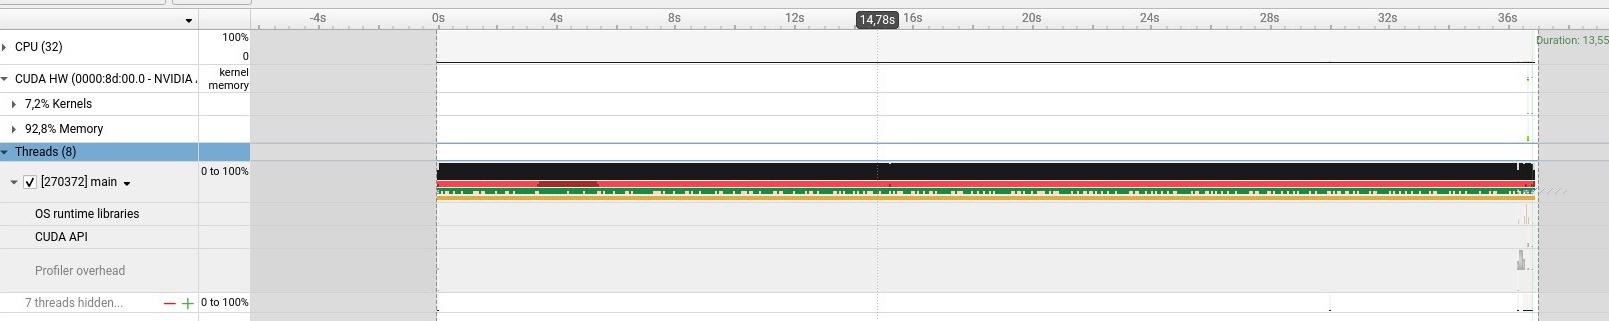
\includegraphics[width=\textwidth]{Images/nsight-all.jpeg}
  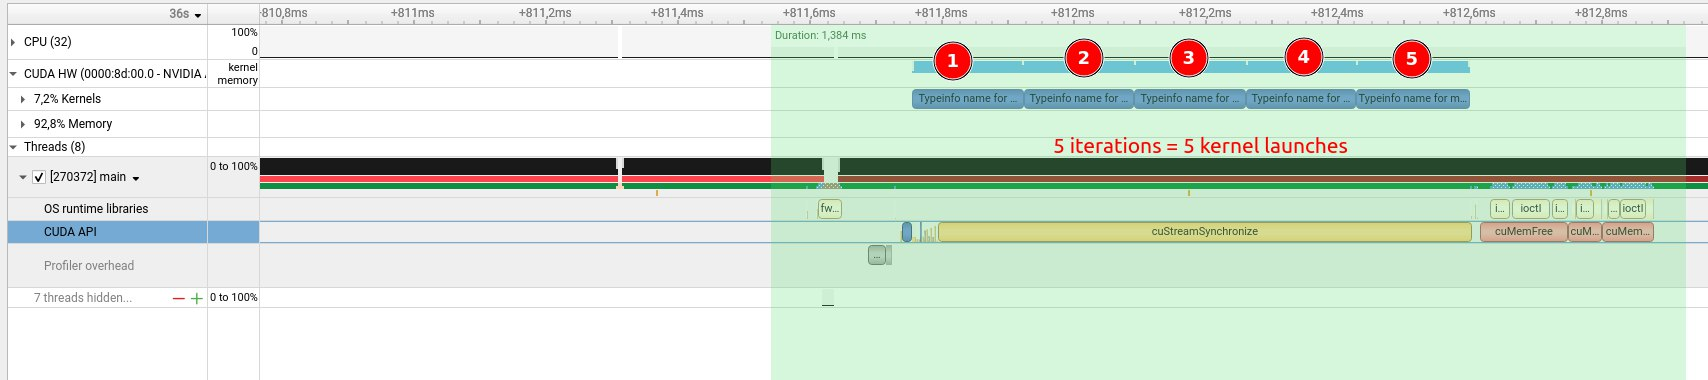
\includegraphics[width=\textwidth]{Images/nsight-kernel.jpeg}
  \end{center}
  \begin{columns}
    \begin{column}{0.48\textwidth}
      Total time: $\sim$37 seconds

      Total kernel time: $\sim$0.008 seconds
    \end{column}
  \end{columns}
\end{frame}
% -------------------------------------------------------------------------
\begin{frame}{Benchmark Comparisons: Backpropagation}
  \begin{center}
  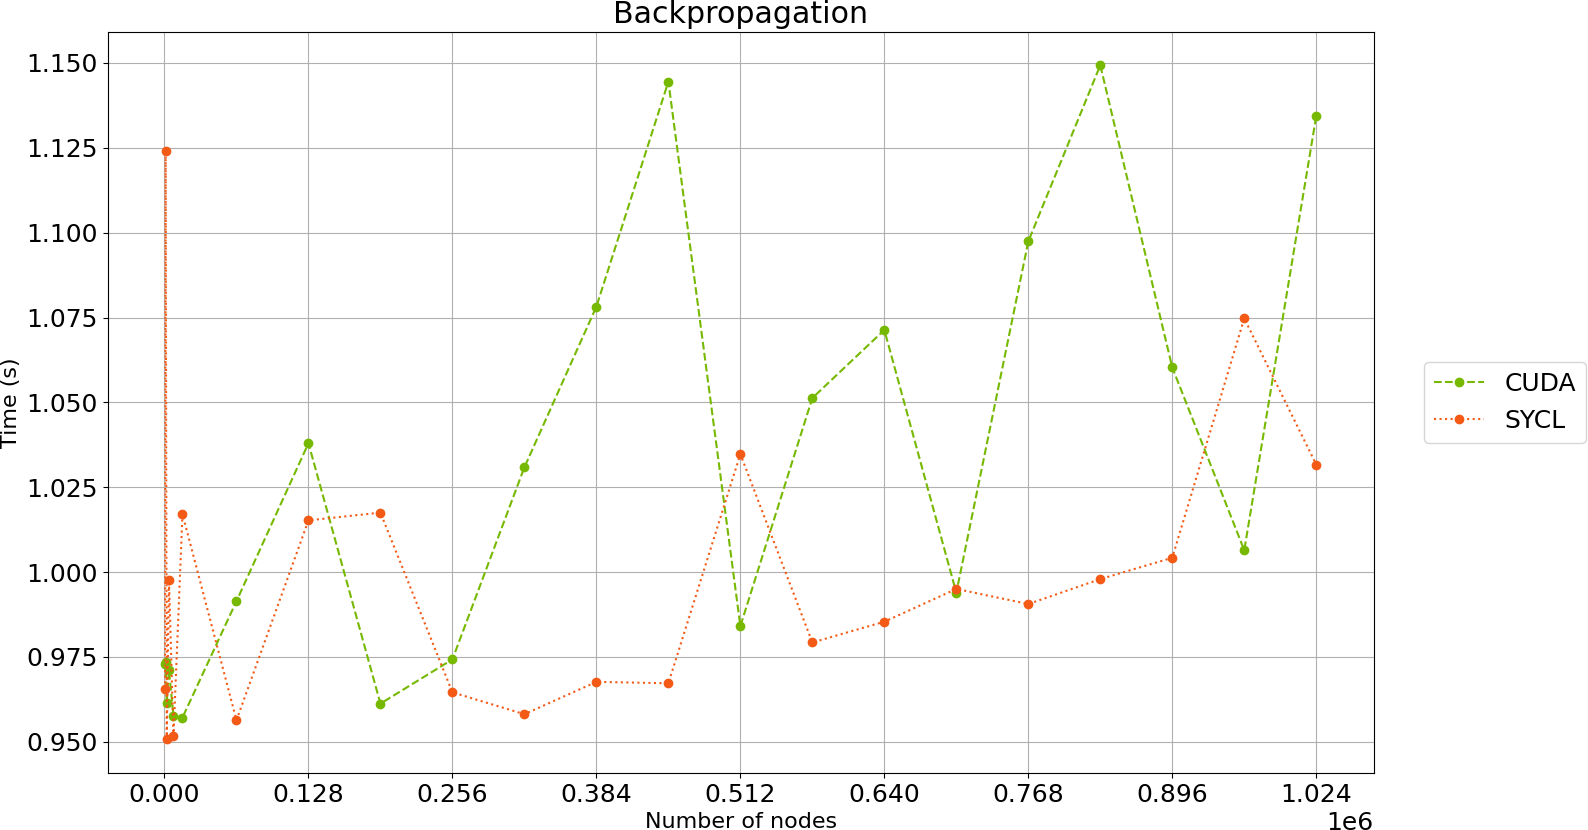
\includegraphics[width=\textwidth]{Images/backprop-sycl-cuda.png}
  \end{center}
\end{frame}
% -------------------------------------------------------------------------

\begin{frame}{Benchmark Comparisons: Backpropagation}
\centering
\lstinputlisting[language=C++,style=cppstyle]{Code/error_backprop_sycl.txt}
NDRange error on backpropagation benchmark
\end{frame}

  \section{An Industry Case Study: Image Processing with SYCL}
  % -------------------------------------------------------------------------
\begin{frame}{An Industry Case Study: Image Processing with SYCL}
  \begin{columns}
    \begin{column}{0.48\textwidth}
      The erosion morphologic operation:
        \begin{itemize}
          \item Lowest value from the neighbourhood
          \item Dark regions get bigger
          \item Bright regions shrink
        \end{itemize}
      \end{column}
      \begin{column}{0.48\textwidth}
        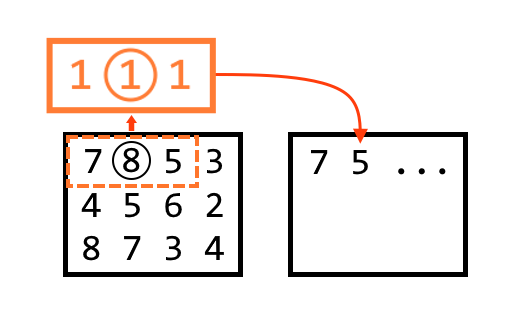
\includegraphics[width=\linewidth]{Images/erosion_graph.png}
      \end{column}
    \end{columns}
    Wooptix proposed to implement this algorithm.
\end{frame}
% -------------------------------------------------------------------------
\begin{frame}{An Industry Case Study: Image Processing with SYCL}
  \lstinputlisting[language=C++,style=cppstyle,title={Partial serial erosion code. \href{{https://github.com/AdrianoMoreira08/TFG-SYCL/blob/main/image-processing/morphology-gray/include/erode.h}}{\textit{See on Github}}}]{Code/serial-morph.cc}
\end{frame}
% -------------------------------------------------------------------------
\begin{frame}{An Industry Case Study: Image Processing with SYCL}
  \lstinputlisting[language=C++,style=cppstyle,title={Memory tiling code for SYCL erosion. \href{{https://github.com/AdrianoMoreira08/TFG-SYCL/blob/main/image-processing/morphology-gray/include/erode_sycl.h}}{\textit{See on Github}}}]{Code/sycl-morph-tile.cc}
\end{frame}
% -------------------------------------------------------------------------
\begin{frame}{An Industry Case Study: Image Processing with SYCL}
  \lstinputlisting[language=C++,style=cppstyle,title={Operation code for SYCL erosion. \href{{https://github.com/AdrianoMoreira08/TFG-SYCL/blob/main/image-processing/morphology-gray/include/erode_sycl.h}}{\textit{See on Github}}}]{Code/sycl-morph-op.cc}
\end{frame}
% -------------------------------------------------------------------------
\begin{frame}{An Industry Case Study: Image Processing with SYCL}
  \begin{figure}[H]
    \centering
    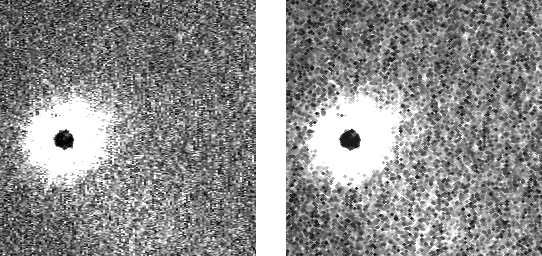
\includegraphics[width=0.7\linewidth]{Images/FOC-result.png}

    Sample from the Faint Object Camera from the Hubble Space Telescope.
    
    Original (left) and eroded (right).
  \end{figure}
  \begin{itemize}
    \item \textbf{Program time}: 1.10 sec. for serial and 1.30 sec. for SYCL
    \item \textbf{Algorithm time}: 0.04 sec. for serial and 0.17 sec. for SYCL
  \end{itemize}
\end{frame}
% -------------------------------------------------------------------------
\begin{frame}{An Industry Case Study: Image Processing with SYCL}
  \begin{figure}[H]
    \centering
    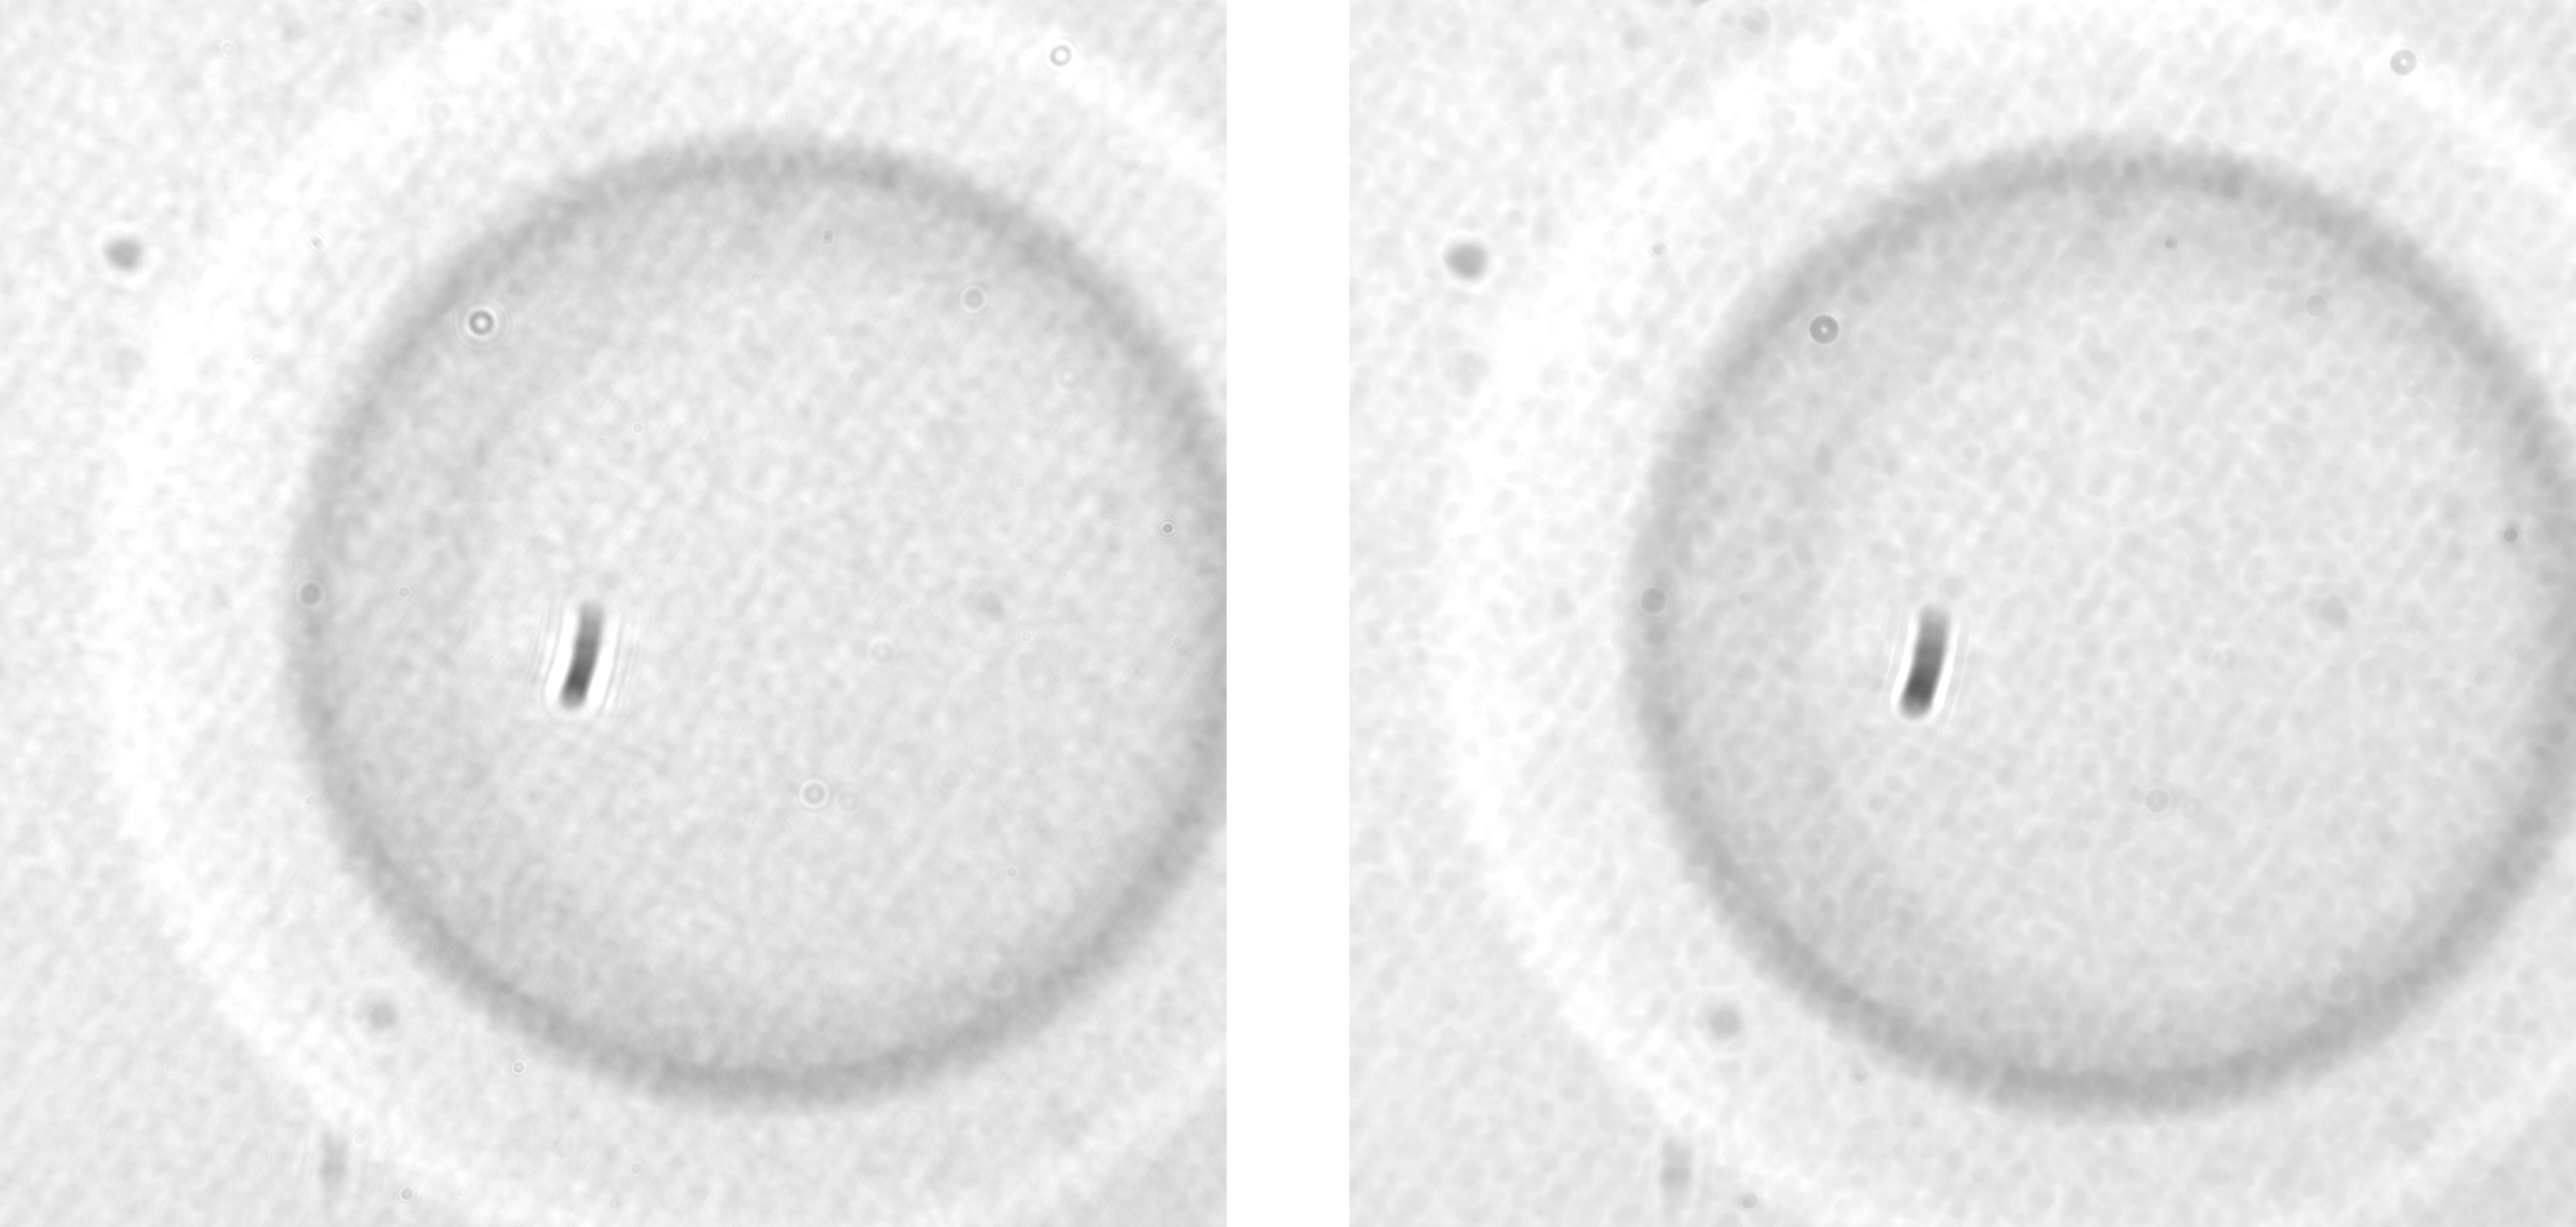
\includegraphics[width=0.7\linewidth]{Images/comparison-wooptix.png}

    Large sample image provided by Wooptix.
    
    Original (left) and eroded (right).
  \end{figure}
  \begin{itemize}
    \item \textbf{Program time}: 58.61 sec. for serial and 56.30 sec. for SYCL
    \item \textbf{Algorithm time}: 3.32 sec. for serial and 0.29 sec. for SYCL
  \end{itemize}
\end{frame}
% -------------------------------------------------------------------------
  \section{Future Work}
  % -------------------------------------------------------------------------
\begin{frame}{Future Work}
\block{Future Work}
  \begin{itemize}
    \item XXX
  \end{itemize}
\endblock{}
\end{frame}
% -------------------------------------------------------------------------

  \section{Summary and conclusions}
  % -------------------------------------------------------------------------
\begin{frame}{Summary and Conclusions}
\block{Summary and Conclusions}
  \begin{itemize}
    \item Contextualization in the field of HPC
    \item Raise the level of knowledge in parallel programming with SYCL
    \item Acquisition of technical knowledge about SYCL
    \item Evaluation of various applications from the HeCBench benchmark collection
    \item Implementation of the erosion operation with SYCL
  \end{itemize}
\endblock{}    
\end{frame}
% -------------------------------------------------------------------------
  % -------------------------------------------------------------------------
\begin{frame} [fragile]
  \frametitle{Thanks for your attention}
  \block{Introduction to High Performance Computing with SYCL}
    \begin{itemize}
    \item {\it GitHub} Repository: \texttt{https://github.com/AdrianoMoreira08/TFG-SYCL}
    \end{itemize}
    \begin{flushright}
    Adriano dos Santos Moreira  \\
    \structure{\footnotesize{adriano.moreira.07@ull.edu.es}}
    \end{flushright}
  \endblock{}
  Thanks also to: \\~\\
  {
  \begin{columns}
    \begin{column}{0.48\textwidth}
      \centering
      
\includegraphics[width=0.4\linewidth]{Images/wooptix-logo.png}
    \end{column}
    \begin{column}{0.1\textwidth}
      {\Large and}
    \end{column}
    \begin{column}{0.48\textwidth}
      \centering
      
\includegraphics[width=0.6\linewidth]{Images/codeplay-logo.png}
    \end{column}
  \end{columns}
  }
\end{frame}
% -------------------------------------------------------------------------
%%%%%%%%%%%%%%%%%%%%%%%%%%%%%%%%%%%%%%%%%%%%%%%%%%%%%%%%%%%%%%%%%%%%%%%%%%%%%%%%%%%%%%%%%
\end{document} 